\setcounter{section}{8}
\section{TP09 - Pushdown Automata (PDAs)}
{
\renewcommand{\thesubsubsection}{\thesubsection\alph{subsubsection}}
\subsection{Exercise 1}
\subsubsection{Item a}
\begin{alignat*}{2}
	S \rightarrow aSb\mid aSbb\mid \varepsilon
\end{alignat*}
\subsubsection{Item b} \label{TP09_1b}
PDA accepting by empty stack.
\begin{center}
\begin{minipage}[c]{0.30\textwidth}
\begin{alignat*}{2}
	PDA    &= (Q, \Sigma, \Gamma, \delta, q_0, Z_0)\\
	Q      &= \{q_0\}\\
	\Sigma &= \{a,b\}\\
	\Gamma &= \{a,b,S\}\\
	Z_0    &= S
\end{alignat*}
\end{minipage}%
\begin{minipage}[c]{0.65\textwidth}
\begin{alignat*}{2}
	\delta \colon & Q \times (\Sigma \cup \{\varepsilon\}) \times (\Gamma \cup \{\varepsilon\}) &&\rightarrow \mathscr{P}(Q \times \Gamma^*))\\
	&\delta(q_0, \varepsilon, S) &&=\{(q_0, aSb), (q_0, aSbb), (q_0, \varepsilon)\}\\
	&\delta(q_0, a, a) &&= \{(q_0, \varepsilon)\}\\
	&\delta(q_0, b, b) &&= \{(q_0, \varepsilon)\}
\end{alignat*}
\end{minipage}
\end{center}
\subsubsection{Item c}
\begin{center} 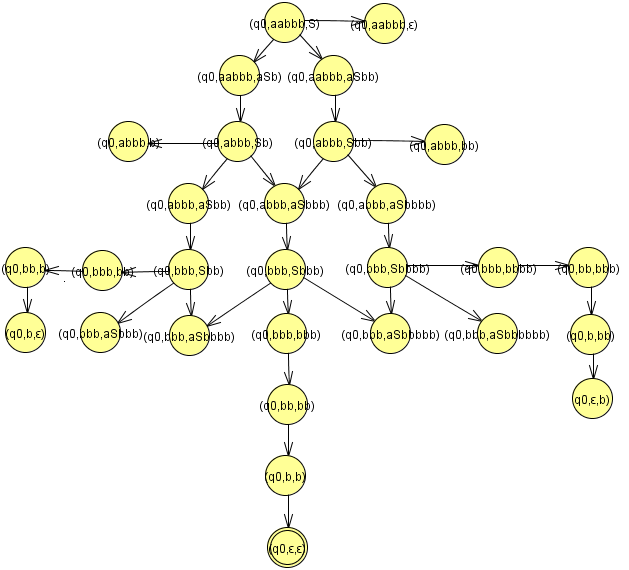
\includegraphics[scale=0.45]{TP09_1c} \end{center}
\pagebreak
\subsubsection{Item d}
When the input string is $aaabb$, the stack has always more $b$'s than can be consumed from the remanescent input.
\begin{center} 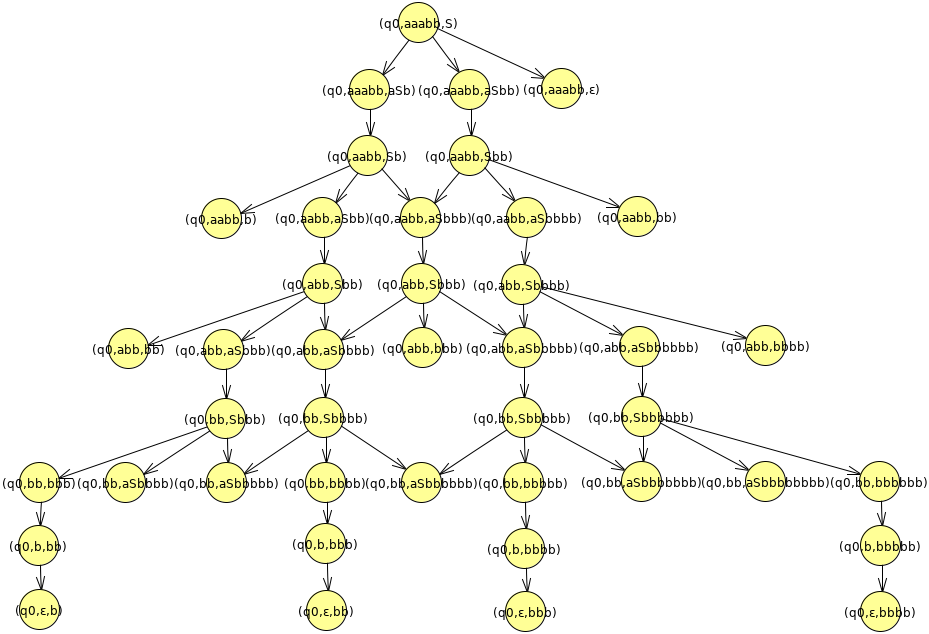
\includegraphics[scale=0.45]{TP09_1d} \end{center}
\subsection{Exercise 2} \label{TP09_2}
\begin{center}
\begin{minipage}[c]{0.30\textwidth}
\begin{alignat*}{2}
	PDA    &= (Q, \Sigma, \Gamma, \delta, q_0, Z_0)\\
	Q      &= \{q_0\}\\
	\Sigma &= \{0,1\}\\
	\Gamma &= \{0,1,S,A\}\\
	Z_0    &= S
\end{alignat*}
\end{minipage}%
\begin{minipage}[c]{0.60\textwidth}
\begin{alignat*}{2}
	\delta \colon Q \times (\Sigma \cup \{\varepsilon\}) \times \Gamma & \rightarrow \mathscr{P}(Q \times \Gamma^*)\\
	\delta(q_0, \varepsilon, S) &= \{(q_0, A1A)\} \\
	\delta(q_0, \varepsilon, A) &= \{(q_0,0A), (q_0, 1A),(q_0,\varepsilon)\}\\
	\delta(q_0, 0, 0) &= \{(q_0, \varepsilon)\}\\
	\delta(q_0, 1, 1) &= \{(q_0, \varepsilon\}
\end{alignat*}
\end{minipage}
\end{center}
\subsection{Exercise 3} \label{TP09_3}
\begin{center}
\begin{minipage}[c]{0.4\textwidth}
\begin{alignat*}{2}
	PDA ~ P &= (Q,\Sigma,\Gamma,\delta, q_0, Z_0)\\
	Q       &= \{q_0\}\\
	\Sigma  &= \{e,i\}\\
	\Gamma  &= \{e,i,S\}\\
	Z_0     &= S
\end{alignat*}
\end{minipage}%
\begin{minipage}[c]{0.6\textwidth}
\begin{alignat*}{2}
	\delta \colon Q \times (\Sigma \cup \{\varepsilon\}) \times \Gamma & \rightarrow \mathscr{P}(Q \times \Gamma ^*)\\
	\delta (q_0,\varepsilon ,S) &=\{(q_0,SS),(q_0,iS),(q_0,iSeS), (q_0, \varepsilon)\}\\
	\delta (q_0,e,e)&=\{(q_0,\varepsilon)\}\\
	\delta (q_0,i,i)&=\{(q_0,\varepsilon)\}
\end{alignat*}
\end{minipage}
\end{center}
\subsection{Exercise 4}
\subsubsection{Item a}
\begin{center} 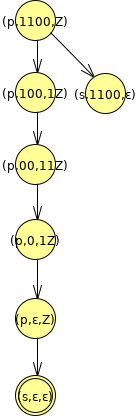
\includegraphics[scale=0.5]{TP09_4a} \end{center}
\subsubsection{Item b}
The string $1100$ is accepted, given this PDA accepts by empty stack, and using it as input the PDA reaches an instantaneous description with empty remanescent input and empty stack.
\subsubsection{Item c}
\begin{center} 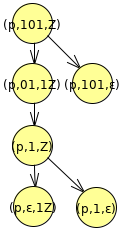
\includegraphics[scale=0.5]{TP09_4c} \end{center}
\subsection{Exercise 5}
This statement is false, given a CFG is ambiguous iff there exists a string with at least two different syntax trees. Having two different syntax trees can be guaranteed by having two different rightmost derivations, or two different leftmost derivations. Having different leftmost and rightmost derivations is not enough to be ambiguous.
}
